\documentclass[ preprint, numerical, superscriptaddress, svgnames,
                amssymb, aps, prb ]{revtex4-2}
\usepackage{graphicx, subcaption, array, booktabs, mathtools, extarrows, tikz,
            physics2, fixdif, bm, derivative, lmodern, amsthm, CJKutf8, url}
\usetikzlibrary{arrows.meta}
\tikzset{> = Stealth}
\newdif \iu {\mathrm i}
\newdif \upe {\mathrm e}
\usepackage[mono = false]{libertine}
\usephysicsmodule{ab, ab.braket, qtext.legacy, op.legacy}
\usepackage[final, nopatch = footnote]{microtype}
\usepackage{silence}
\WarningFilter{revtex4-2}{Repair the float}
\bibliographystyle{apsrev4-2}
\usepackage{etoolbox, zref-clever, zref-titleref}
\zcsetup{cap, abbrev}
\makeatletter
\patchcmd{\frontmatter@abstract@produce}
  {\vskip200\p@\@plus1fil
   \penalty-200\relax
   \vskip-200\p@\@plus-1fil}{}{}{}
\makeatother

\begin{document}

\title{Band Structure Calculations of Two-dimensional Kagome Lattice by Tight
  Binding Model}
\author{Mingyu Xia (夏明宇)}
\email{\ttfamily xiamingyu@westlake.edu.cn}
\affiliation{Department of Physics, Westlake University}
\date{2026-01-04 --- Final Project of PHY4804}

\begin{CJK*}{UTF8}{gbsn}
\maketitle
\end{CJK*}

\section{Introduction}

The kagome lattice in this sense consists of the vertices and edges of the
trihexagonal tiling~\cite{WikipediA}.

Different from the two type of sites in Honeycomb lattice, the Kagome lattice
has 3 types of sites, \textcolor{blue}{$A$ (blue)}, \textcolor{red}{$B$ (red)},
and \textcolor{Green}{$C$ (green)}, respectively.
\begin{figure}[htbp]
  \begin{minipage}[t]{.48\linewidth}
    \centering
    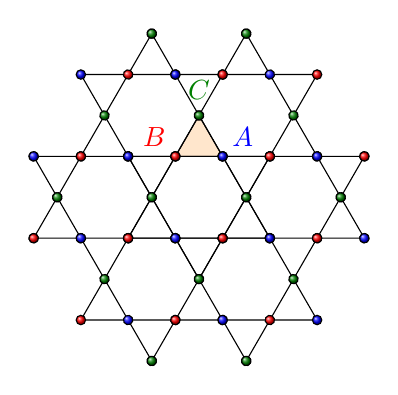
\begin{tikzpicture}[scale = .6]
      \fill [orange, opacity = .2]
        (.5,{sqrt(3)}) node [opacity = 1, blue, above right] {$A$} --++
        (-1,0) node [opacity = 1, red, above left] {$B$} --++
        (60:1) node [opacity = 1, Green, above = .5ex] {$C$} -- cycle;
      \foreach \i in {0, 180}
        {
      \begin{scope}[rotate around = {\i:(0,{sqrt(3)/2})}]
        \draw (-3.5,0) --++ (5,0) --++ (120:5) --++ (240:5) -- cycle;
        \draw (-1.5,0) --++ (5,0) --++ (120:5) --++ (240:5) -- cycle;
        \draw (-2.5,{-sqrt(3)}) --++ (5,0) --++ (120:5) --++ (240:5) -- cycle;
      \end{scope}
        }
      \foreach \i in {0, 180}
        {
      \begin{scope}[rotate around = {\i:(0,{sqrt(3)/2})}]
        \foreach \j in {0, 2}
        {
      \begin{scope}[xshift = \j cm]
        \shade [draw, ball color = blue] (-2.5,0) circle (.1);
        \shade [draw, ball color = blue] (-.5,0) circle (.1);
        \shade [draw, ball color = blue] (1.5,0) circle (.1);
        \shade [draw, ball color = red] (-3.5,0) circle (.1);
        \shade [draw, ball color = red] (-1.5,0) circle (.1);
        \shade [draw, ball color = red] (.5,0) circle (.1);
        \begin{scope}[rotate around = {60:(-3.5,0)}]
          \shade [draw, ball color = red] (-3.5,0) circle (.1);
          \shade [draw, ball color = red] (-1.5,0) circle (.1);
          \shade [draw, ball color = red] (.5,0) circle (.1);
          \shade [draw, ball color = Green] (-2.5,0) circle (.1);
          \shade [draw, ball color = Green] (-.5,0) circle (.1);
          \shade [draw, ball color = Green] (1.5,0) circle (.1);
        \end{scope}
        \begin{scope}[rotate around = {-60:(1.5,0)}]
          \shade [draw, ball color = Green] (-3.5,0) circle (.1);
          \shade [draw, ball color = Green] (-1.5,0) circle (.1);
          \shade [draw, ball color = Green] (.5,0) circle (.1);
          \shade [draw, ball color = blue] (-2.5,0) circle (.1);
          \shade [draw, ball color = blue] (-.5,0) circle (.1);
          \shade [draw, ball color = blue] (1.5,0) circle (.1);
        \end{scope}
        \shade [draw, ball color = red] (-2.5,{-sqrt(3)}) circle (.1);
        \shade [draw, ball color = blue] (.5,{-sqrt(3)}) circle (.1);
      \end{scope}
        }
      \end{scope}
        }
    \end{tikzpicture}
  \end{minipage}
  \hfill
  \begin{minipage}[t]{.48\linewidth}
    \centering
    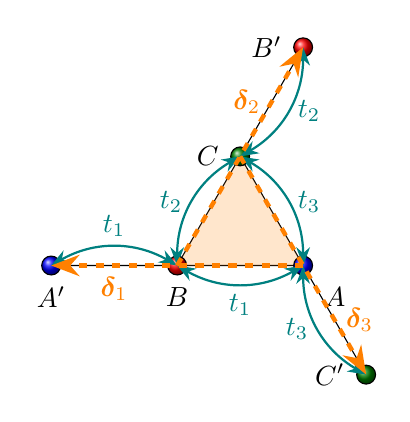
\begin{tikzpicture}[scale = .8]
      \draw (2,0) -- (-2,0)
            (0,0) -- (2,{2*sqrt(3)})
            (1,{sqrt(3)}) -- (3,{-sqrt(3)});
      \fill [orange, opacity = .2] (0,0) -- (1,{sqrt(3)}) -- (2,0) -- cycle;
      \shade [draw, ball color = blue] (2,0) circle (.15) coordinate (A)
       node [below right = .15cm] {$A$};
      \shade [draw, ball color = red] (0,0) circle (.15) coordinate (B)
       node [below = .15cm] {$B$};
      \shade [draw, ball color = Green] (1,{sqrt(3)}) circle (.15)
       coordinate (C) node [left = .15cm] {$C$};

      \shade [draw, ball color = blue] (-2,0) circle (.15)
       coordinate (A') node [below = .15cm] {$A'$};
      \shade [draw, ball color = red] (2,{2*sqrt(3)}) circle (.15)
       coordinate (B') node [left = .15cm] {$B'$};
      \shade [draw, ball color = Green] (3,{-sqrt(3)}) circle (.15)
       coordinate (C') node [left = .15cm] {$C'$};
      \draw [thick, <->, teal] (A) to[bend left] node [below] {$t_1$} (B);
      \draw [thick, <->, teal] (B) to[bend left] node [left] {$t_2$} (C);
      \draw [thick, <->, teal] (C) to[bend left] node [right] {$t_3$} (A);
      \draw [thick, <->, teal] (B) to[bend right] node [above] {$t_1$} (A');
      \draw [thick, <->, teal] (C) to[bend right] node [right] {$t_2$} (B');
      \draw [thick, <->, teal] (A) to[bend right] node [left] {$t_3$} (C');
      \draw [ultra thick, dashed, ->, orange] (B) --
       node [left, near end] {$\bm \delta_2$} (B');
      \draw [ultra thick, dashed, ->, orange] (A) --
       node [below, near end] {$\bm \delta_1$} (A');
      \draw [ultra thick, dashed, ->, orange] (C) --
       node [right, near end] {$\bm \delta_3$} (C');
    \end{tikzpicture}
  \end{minipage}
  \caption{Top view of the Kagome Lattice and
    tight-binding model with the NN hopping}
  \zlabel{fig:Kagome}
\end{figure}
The three sites in the unit cell form a regular triangle, which is shaded
in~\zcref{fig:Kagome}.
If we simplify taking the unit cell located at $\bm r$. Then, each site in the
unit cell has 2 NN hoppings, pointing out by the lattice vectors
\begin{equation}
  \bm \delta_1 = a(-2,0),     \quad
  \bm \delta_2 = a(1, \sqrt3),\quad
  \bm \delta_3 = a(1,-\sqrt3).
\end{equation}
where $a$ is the lattice constant, the distance between any two NN lattices.

\section{Model Hamiltonian}

In this model, consider the nearest-neighbor (NN) hopping with different
hopping magnitude $t_1$, $t_2$, and $t_3$.
The Hamiltonian illustrates the tight-binding model in terms of second
quantization
\begin{equation}
  \mathcal H = -\sum_{\bm r}[
    t_1(a_{\bm r}^\dagger b_{\bm r} + b_{\bm r}^\dagger a_{\bm r+\bm\delta_1})
  + t_2(b_{\bm r}^\dagger c_{\bm r} + c_{\bm r}^\dagger b_{\bm r+\bm\delta_2})
  + t_3(c_{\bm r}^\dagger a_{\bm r} + a_{\bm r}^\dagger c_{\bm r+\bm\delta_3})]
  + \text{H.c.}
\end{equation}
Assume there are $N$ $A$-, $B$-, and $C$- type sites in total.
Applying the Fourier transformation to the Fermion operators
\begin{alignat*}{3}
  & \hat a_i
  = \frac1{\sqrt N} \sum_{\bm k} \upe^{\iu \bm k\cdot \bm r_i} \hat a_{\bm k},
  &\hspace*{2\arraycolsep}
  & \hat b_i
  = \frac1{\sqrt N} \sum_{\bm k} \upe^{\iu \bm k\cdot \bm r_i} \hat b_{\bm k},
  &\hspace*{2\arraycolsep}
  & \hat c_i
  = \frac1{\sqrt N} \sum_{\bm k} \upe^{\iu \bm k\cdot \bm r_i} \hat c_{\bm k},\\
  & \hat a_{i+\bm\delta_1}
  = \frac1{\sqrt N} \sum_{\bm k}
    \upe^{\iu \bm k\cdot (\bm r_i + \bm \delta_1)} \hat b_{\bm k},
& & \hat b_{i+\bm\delta_2}
  = \frac1{\sqrt N} \sum_{\bm k}
    \upe^{\iu \bm k\cdot (\bm r_i + \bm \delta_2)} \hat b_{\bm k},
& & \hat c_{i+\bm\delta_3}
  = \frac1{\sqrt N} \sum_{\bm k}
    \upe^{\iu \bm k\cdot (\bm r_i + \bm \delta_3)} \hat c_{\bm k}.
\shortintertext{Similar for their Hermite conjugates}
  & \hat a_i^\dagger
  = \frac1{\sqrt N} \sum_{\bm k}
    \upe^{-\iu \bm k\cdot \bm r_i} \hat a_{\bm k}^\dagger,
& & \hat b_i^\dagger
  = \frac1{\sqrt N} \sum_{\bm k}
    \upe^{-\iu \bm k\cdot \bm r_i} \hat b_{\bm k}^\dagger,
& & \hat c_i^\dagger
  = \frac1{\sqrt N} \sum_{\bm k}
    \upe^{-\iu \bm k\cdot \bm r_i} \hat c_{\bm k}^\dagger,\\
  & \hat a_{i+\bm\delta_1}^\dagger
  = \frac1{\sqrt N} \sum_{\bm k}
    \upe^{-\iu \bm k\cdot (\bm r_i + \bm \delta_1)} \hat a_{\bm k}^\dagger,
& & \hat b_{i+\bm\delta_2}^\dagger
  = \frac1{\sqrt N} \sum_{\bm k}
    \upe^{-\iu \bm k\cdot (\bm r_i + \bm \delta_2)} \hat b_{\bm k}^\dagger,
& & \hat c_{i+\bm\delta_3}^\dagger
  = \frac1{\sqrt N} \sum_{\bm k}
    \upe^{-\iu \bm k\cdot (\bm r_i + \bm \delta_3)} \hat c_{\bm k}^\dagger.
\end{alignat*}
Substituting the transformed operators into the Hamiltonian, one can
obtain $\mathcal H
= \sum_{\bm k} \Psi_{\bm k}^\dagger \tilde{\mathcal H} \Psi_{\bm k}$,
where
\begin{equation}
  \tilde{\mathcal H} =-
  \begin{pmatrix}
    0 & t_1(1 + \upe^{\iu k_1}) & t_2(1 + \upe^{\iu k_2})\\
    t_1(1 + \upe^{-\iu k_1}) & 0 & t_3(1 + \upe^{-\iu k_3})\\
    t_2(1 + \upe^{\iu k_2}) & t_3(1 + \upe^{\iu k_3}) & 0
  \end{pmatrix}.
\end{equation}

\section{Advanced: The Next-Nearest Neighbor Hopping Term}

The totla Hamiltonian can be separated into two terms: The NN
(Nearest neighbor) one and the NNN (Next-Nearest Neighbor) one
\begin{equation}
  \mathcal H' = \mathcal H_\text{NN} + \mathcal H_\text{NNN},
\end{equation}
with the two terms in second quantization form
\begin{gather}
  \mathcal H_\text{NN} =,\\
  \mathcal H_\text{NNN} =.
\end{gather}

Hamiltonian matrix in momentum space
\begin{equation}
  \tilde{\mathcal H}' =-
  \begin{pmatrix}
    \epsilon_A & t_1(1 + \upe^{\iu k_1}) & t_2(1 + \upe^{\iu k_2})\\
    t_1(1 + \upe^{-\iu k_1}) & \epsilon_B & t_3(1 + \upe^{-\iu k_3})\\
    t_2(1 + \upe^{\iu k_2}) & t_3(1 + \upe^{\iu k_3}) & \epsilon_C
  \end{pmatrix}.
\end{equation}

\clearpage

\bibliography{reference}

\end{document}